\chapter{Transmissão em série de dados HDMI} \label{chap:chap5}

%imp -> https://www.xilinx.com/support/answers/64340.html
Neste capítulo são contempladas todas as arquiteturas desenvolvidas para a transmissão dos dados HDMI em série, explicando todas as decisões tomadas para se obter o produto final. 

\section{Abordagem inicial}

Numa fase inicial do projeto optou-se por abordar de uma maneira simples a transmissão dos dados em série, sem o recurso à definição de todas a tramas de uma pacote. Tal decisão foi tomada, ciente da importância das tramas num protocolo de comunicação, pois o módulo GTX disponibilizado pela \textit{Xilinx} é muito complexo e completo e foi necessário uma familiarização com o mesmo.

\subsection{Transmissão de uma barra de cores gerada na FPGA em série} \label{sub:planD}

A arquitetura desenvolvida passa por um conjunto de fases que vão desde a criação do módulo GTX através da interface disponibilizada no \textit{software} para tal, e todas as tomadas de decisões que isso envolve, até a concepção de arquiteturas que criem e verifiquem as tramas. Todas essas fases serão devidamente explicadas nesta subsecção.

\subsubsection{Considerações sobre a arquitetura} \label{subsub:planD_considerações}

A arquitetura desenvolvida gera uma barra de cores em \textit{FULL HD} na FPGA, tal como descrito em \ref{subsub:planA} no capítulo \ref{chap:chap3}, a uma taxa de atualização vertical de 60 Hz. A placa HDMI transmissora utilizada nesta arquitetura deve receber imagens no formato RGB de 30 bits e por isso está programada para a configuração por omissão, referida em \ref{subsubsec:HDMIconfigdefault} na página \pageref{subsubsec:HDMIconfigdefault}. Para além disto, a arquitetura também tem um bloco que gera as tramas e envia-as para o GTX, do mesmo modo que tem um bloco que recebe as tramas e retira a informação das mesmas, enviando-as para uma arquitetura que envie esses mesmos dados para a placa HDMI transmissora. Este diagrama geral da arquitetura esta representado na figura \ref{fig:planD_SIMPLES}.

\begin{figure}[h!]
	\begin{center}
		\leavevmode
		\includegraphics[width=1.0\textwidth]{planod_simples}
		\captionsetup{width=1.0\linewidth}
		\caption[Diagrama de blocos geral da arquitetura que transmite uma barra de cores em série]{Diagrama de blocos geral da arquitetura que transmite uma barra de cores em série}
		\label{fig:planD_SIMPLES}
	\end{center}
\end{figure}

Tal como é de esperar, e foi referido em \ref{sec:sincronizacao} na página \pageref{sec:sincronizacao}, os sinais de relógio provenientes do GTX e do módulo que gera a barra de cores não são o mesmo, e por isso, existe um bloco entre a geração e a criação de tramas que permite a sincronização entre os diferentes domínios de sinais de relógio através de \textit{shift-registers}.

Tendo em conta a arquitetura global desenvolvida, foram tomadas 2 decisões importantes para definir as características do transcetor: o número de bits por trama e a frequência a que estas serão lidas para o mesmo. Tal como já foi referido, a maneira mais eficiente no que toca à escolha da frequência de amostragem para o transcetor, é escolher a própria frequência da imagem HDMI, ou seja, 148,5 MHz para uma imagem \textit{FULL HD}. Relativamente ao número de bits por trama, tendo em conta que é necessário enviar os sinais todos (\textit{pixel}, \textit{vsync}, \textit{hsync} e \textit{enable}) e visto que nesta fase do projeto não houve a preocupação da criação de diferentes tramas para os diversos momentos de transmissão, escolheu-se enviar tramas de 40 bits.

Observando novamente a tabela \ref{table:line_rates} na página \pageref{table:line_rates}, independentemente do tamanho do \textit{datapath} escolhido, obtém-se uma taxa de transmissão de dados de 5,94 Gb/s.

\subsubsection{Geração do Módulo GTX} \label{subsub:GTX_generate}

Quando se gera o módulo GTX através da interface disponibiliza pelo \textit{software} VIVADO existem algumas decisões que necessitam de ser tomadas para além das que já foram. Essas passam de seguida a ser detalhadas:

Do lado do transmissor tomaram-se as seguintes principais decisões:
\begin{enumerate}
%	\item \textbf{\textit{Line Rate:}} Como referido anteriormente é 5,94 Gb/s.
%	\item \textbf{Frequência de Amostragem das Tramas:} Assim como referido anteriormente é 148,5 MHz.
%	\item \textbf{Tamanho da interface com a FPGA:} Tal como explicado em \ref{subsub:planD_considerações} na página \pageref{subsub:planD_considerações} é 40 bits
	\item \textbf{Tamanho interno dos dados:} Esta escolha envolve o número de \textit{datapath} que são utilizados e ainda o valor da frequência de TXUSRCLK. Foi selecionado 40 bits o que implica o uso de apenas um \textit{datapath} e obtém-se as frequências de TXUSRCLK E TXUSRCLK2 idênticas.
	\item \textbf{Tipo de codificação:} Neste caso não se escolheu codificação porque não é possível (a interface com a FPGA é de 40 bits) e também numa fase inicial optou-se por simplificar o projeto.
	\item \textbf{Escolha ente \textit{Buffer} ou Bloco de Alinhamento de Fase:} Tal como indicado na secção \ref{subsub:tx_buffer} foi escolhido a utilização do \textit{buffer} uma vez que é de mais fácil utilização não requerendo o uso de lógica extra (comparativamente ao bloco de alinhamento de fase) e ainda assim é robusto.
\end{enumerate}

Do lado do recetor as principais decisões tomadas foram as seguintes:
\begin{enumerate}
	\item \textbf{Tipo de equalização:} Na subsecção \ref{subsub:rx_equalização} são apresentadas as vantagens de cada um dos tipos de equalizadores disponíveis. Apesar de este ser um projeto simples em que não se pretende inserir o sinal em canais ruidosos, optou-se por utilizar um equalizador DFE uma vez que traz mais vantagens do a utilização do equalizador LPM.
	\item \textbf{Alinhamento de palavras:} Como palavra de alinhamento escolheu-se o caractere K28.3 da tabela \ref{table:caracteres_especiais_8b10b} na página \pageref{table:caracteres_especiais_8b10b}. Contudo é necessário ter em conta que não se está a utilizar codificação e, como tal, para efetuar o alinhamento da palavra o recetor não alinhará pelo caractere K28.3 codificado, mas sim, não codificado. Ou seja, na realidade quando encontrar a palavra "7C" assume que é a palavra de alinhamento e alinha a trama para esse limite. Para além disso, optou-se por ativar a porta "RXSLIDE" que ativa o alinhamento manual dos bits, pois tal como referido em \ref{subsub:align} é de esperar que seja necessário ativar o alinhamento manual para ligações cuja taxa de débito seja superior a 5 Gb/s.
	\item \textbf{Tipo de descodificação:} Não foi utilizada nenhuma descodificação, pois do lado do transmissor também não há codificação.
	\item \textbf{Escolha ente \textit{Buffer} ou Bloco de Alinhamento de Fase:} Optou-se pela escolha do \textit{buffer}, porque no caso do recetor para além não requerer lógica extra e ter uma inicialização mais rápida (comparativamente ao bloco de alinhamento de fase), também não exige que a correcção do sinal de relógio seja realizada fora do transcetor, tal como mencionado em \ref{subsub:rx_buffer}.
\end{enumerate}

Na tabela \ref {table:sumario_planoD} é apresentada uma tabela sumário do módulo gerado. Esta tabela foi adaptada da interface que gera o módulo.

\begin{table}[h!]
	\centering
	\begin{tabular}{@{}ll@{}}
		\toprule
		\multicolumn{1}{c}{\textbf{Característica}} & \multicolumn{1}{c}{\textbf{GT}} \\ \midrule
		\textbf{TX Line Rate (Gb/s)}                & 5,94                            \\
		\textbf{TX Reference Clock (MHz)}           & 148,5                           \\
		\textbf{Enconding}                          & None                            \\
		\textbf{TX Internal Data Width}             & 40                              \\
		\textbf{TX External Data Width}             & 40                              \\
		\textbf{TXUSRCLK (MHz)}                     & 148,5                           \\
		\textbf{TXUSRCLK2 (MHz)}                    & 148,5                           \\
		\textbf{TX Buffer Enabled}                  & TRUE                            \\
		\textbf{RX Line Rate (Gb/s)}                & 5,94                            \\
		\textbf{RX Reference Clock (MHz)}           & 148,5                           \\
		\textbf{Decoding}                           & None                            \\
		\textbf{RX Internal Data Width}             & 40                              \\
		\textbf{RX External Data Width}             & 40                              \\
		\textbf{RXUSRCLK (MHz)}                     & 148,5                           \\
		\textbf{RXUSRCLK2 (MHz)}                    & 148,5                           \\
		\textbf{RX Buffer Enabled}                  & TRUE                            \\ \bottomrule
	\end{tabular}
	\caption[Sumário do módulo GTX gerado para a transmissão de uma barra de cores gerada na FPGA]{Sumário do módulo GTX gerado para a transmissão de uma barra de cores gerada na FPGA (adaptada do \textit{software})}
	\label{table:sumario_planoD}
\end{table}

\subsubsection{Concepção e Desenvolvimento}

Na imagem \ref{fig:planD_SIMPLES} da página \pageref{fig:planD_SIMPLES} é representado um protótipo da arquitetura geral apresentada. Nesta subsecção são apresentados com detalhe todos os blocos utilizados e suas entradas e saídas para que se possa perceber as ligações entre os mesmos. 

\subsubsection*{Bloco gerador de uma Barra de Cores} \label{subsub:serial_colorBarGenerator}

Este bloco gerador de barra de cores é exatamente igual ao bloco descrito em \ref{subsub:planA} na página \pageref{subsub:planA}: gera uma barra de cores em \textit{FULL HD} com uma frequência de 148,5 MHz. Nas suas entradas encontram-se as portas vindas diretamente do exterior, tal como nas outras arquiteturas que utilizam este bloco, que são botões definidos pelo utilizador (\textit{reset} e \textit{start}) e também um sinal de relógio diferencial de 200 MHz. Este bloco coloca nas suas saídas sinais que são enviados para um bloco sincronizador dos dados HDMI que é de seguida detalhado.

\subsubsection*{Bloco Sincronizador dos dados HDMI} \label{subsub:serial_syncsignals}

O recurso a este bloco sincronizador dos dados HDMI é necessário devido aos diferentes domínios de relógio que existem no sistema: por um lado existe um bloco que gera uma barra de cores a uma determinada cadência, e por outro existe um bloco que gera as tramas a serem enviadas para o transcetor a outra cadência. Estes dois sinais de relógio podem ser iguais, no entanto podem não estar em fase o que é suficiente para haver problemas de meta-estabilidade. 

Por este motivo, este bloco de sincronização é apenas constituído por dois registos de deslocamento (\textit{shift-registers}) para que problemas de sincronização que possam eventualmente existir sejam resolvidos, tal como apresentado na figura \ref{fig:sync_block}. 
\begin{figure}[h!]
	\begin{center}
		\leavevmode
		\includegraphics[width=0.5\textwidth]{sync_block_from_HDMI}
		\captionsetup{width=1.0\linewidth}
		\caption[Bloco de sincronização de dados]{Bloco de sincronização de dados}
		\label{fig:sync_block}
	\end{center}
\end{figure}

Tal como se visualiza na figura, para além de nas suas entradas se encontrar os dados provenientes da fonte HDMI (que nesta arquitetura é o bloco gerador de barra de cores), há também dois sinais : \textit{rst} e \textit{sys\_rst}. O primeiro sinal refere-se ao sinal de \textit{reset} controlado pelo utilizador e o segundo corresponde a um sinal de \textit{reset} ativado automaticamente pelo módulo GTX.

O sinal de relógio a que opera este bloco trata-se do sinal de relógio proveniente do módulo GTX, tal como se visualiza na figura \ref{fig:planD_SIMPLES} na página \pageref{fig:planD_SIMPLES}.

\subsubsection*{Gerador de Tramas} \label{subsub:serial_frameGenerator}

Este bloco é responsável pela criação das tramas de 40 bits a serem enviadas para o módulo GTX. Relembra-se que nesta abordagem inicial do projeto não se teve em conta a criação de tramas bem definidas para todos os momentos de transição, apenas se definiu a trama que corresponde ao início de transmissão para que fosse possível do lado do recetor manter o alinhamento das tramas. 

%%Explicar trama de SOP, qdo é enviada e pq tem aquele padrão
A trama que define o início da transmissão (SOP - \textit{Start of Packet}) é uma trama que serve essencialmente para o alinhamento das palavras do lado do recetor. Ou seja, são aproveitados momentos de transmissão nulos para enviar esta trama e alinhar a mesma. Isto porque neste momento se está a lidar com uma taxa de transmissão superior a 5 Gb/s e por isso é de esperar que é necessário do lado do recetor verificar se as tramas estão realmente alinhadas.
Esta trama SOP são 40 bits que em hexadecimal corresponde a: $000605047c$. Para além de ter sido a trama de SOP sugerida pelo exemplo que a \textit{Xilinx} disponibiliza, esta trama tem as seguintes particularidades:
\begin{enumerate}
	\item No final da mesma se encontra a palavra de alinhamento(são os primeiros bits a ser transmitidos), que permite ao transcetor alinhar a trama internamente.
	\item A trama numa vista geral nunca será encontrada no meio de outros dados, que será de seguida explicado
\end{enumerate}

Esta trama é transmitida sempre que os sinais de controlo se encontram inativos, ou seja que as seguintes condições se verificarem:
\begin{enumerate}
	\item $vsync = 0$
	\item $hsync = 0$
	\item $enable = 0$
\end{enumerate}


%%Explicar como são os pacotes noutras alturas de transmissão sem ser qdo se envia SOP
Quando estas três condições não se verificam em conjunto, então é porque há algum sinal de imagem ativo, e por isso é transmitida uma trama com o formato que se visualiza na figura \ref{fig:trama_abordagem_inicial}.

\begin{figure}[h!]
	\begin{center}
		\leavevmode
		\includegraphics[width=0.9\textwidth]{trama_abordagem_inicial}
		\captionsetup{width=1.0\linewidth}
		\caption[Estrutura das tramas geradas]{Estrutura das tramas geradas}
		\label{fig:trama_abordagem_inicial}
	\end{center}
\end{figure}

Este formato de trama vem validar aquilo que foi dito anteriormente quando se justificou o formato da trama SOP: os últimos 7 bits da trama SOP são $1111100$, enquanto que os últimos 7 bits de todas as outras tramas são $1010101$. Portanto, em conjunto com o bloco verificador de tramas que garante que as tramas estão sempre alinhadas, dificilmente a trama SOP será encontrada no meio dos dados transmitidos enquanto dados da transmissão e não como trama de alinhamento.


Assim sendo, consoante os dados que recebe nas suas entradas (\textit{pixel}, \textit{vsync}, \textit{hsync} e \textit{enable}), este bloco ou envia SOP ou envia tramas no formato da imagem \ref{fig:trama_abordagem_inicial}. A imagem \ref{fig:momentos_tramas} exemplifica os diversos momentos de transmissão das diferentes tramas numa imagem. A cinza correspondem os momentos da imagem em que os sinais de controlo estão inativos, e por isso são transmitidos SOP, e a castanho correspondem os momentos de transmissão em que algum dos sinais de controlo está ativo e por isso são enviadas tramas no formato previamente exemplificado. Sempre o sinal \textit{rst} ou \textit{sys\_rst} estiver ativo então os dados são repostos e as tramas enviadas são SOP. 

\begin{figure}[h!]
	\begin{center}
		\leavevmode
		\includegraphics[width=0.7\textwidth]{exemplo_tramas_transmissoes}
		\captionsetup{width=1.0\linewidth}
		\caption[Momentos de transmissão de diferentes tramas]{Momentos de transmissão de diferentes tramas}
		\label{fig:momentos_tramas}
	\end{center}
\end{figure}

É de esperar que a transmissão demore algum tempo a alinhar do lado do recetor, e por isso, é necessário que as tramas SOP sejam enviadas durante algum tempo, por isso se escolheram os momentos de transição de dados de controlo nulos, pois são suficientemente longos para que as tramas possam ser alinhadas. Assim, no pior dos casos, perde-se a primeira imagem completa que é transmitida, pois não são recebidos os primeiros dados de controlo (\textit{vsync} e \textit{hsync}) mas garanta-se que todas as outras estão alinhadas e os dados serão corretamente recebidos do lado do transmissor.

\subsubsection*{Verificador de Tramas} \label{subsub:serial_frameChecker}
  
%%Explicar porque existe

Este bloco é responsável pela re-organização das tramas recebidas que são recebidas à cadência RXUSRCLK2. Apesar de poder parecer que com o alinhamento interno as tramas chegariam ao recetor tal como são enviadas do transmissor, mesmo com o alinhamento interno ideal, tal não acontece. As tramas são alinhadas para um determinado limite assim que o recetor encontra as palavra de alinhamento, no entanto não significa que a trama recebida é exatamente à trama enviada. 

O que o alinhamento interno faz, segundo \cite{R022} e \cite{R011}, quando deteta a palavra de alinhamento é assumir que dessa palavra para a frente são dados válidos, tal como explicado anteriormente, e alinhar os dados para um determinado limite. Esse limite pode ser selecionado aquando a criação do módulo na interface especifica para tal, e o que foi escolhido é que alinha os dados para o byte mais próximo. Apesar de não se estar a lidar com codificação, o bloco de alinhamento das palavras considera que 1 byte são 10 bits (pois com a codificação 8B/10B codifica 8 bits em 10 bits) porque o \textit{datapath} é de 40 bits, e por isso quando deteta a palavra de alinhamento, as tramas recebidas no recetor podem chegar de 4 maneiras diferentes ilustradas na imagem \ref{fig:alinhamento_tramas_gtx}.


%Se o datapath fosse de 32 bits sem codificação, assumiria que 1 byte sao 8 bits, de certeza, apesar de eu nao ter testado
\begin{figure}[h!]
		\begin{center}
		\leavevmode
		\includegraphics[width=0.8\textwidth]{organizacao_tramas}
		\captionsetup{width=1.0\linewidth}
		\caption[Alinhamento das tramas no transcetor]{Alinhamento das tramas no transcetor}
		\label{fig:alinhamento_tramas_gtx}
	\end{center}
\end{figure}

Daí a importância da trama de SOP: quando é detetada em algum dos limites assinalados a cinzento dá-se inicio à transmissão dos restantes dados. Para se proceder à organização dos dados recebidos é necessário recorrer a uma máquina de estados. Esta máquina de estados utilizada neste exemplo foi adaptada de uma disponibilizada pela \textit{Xilinx}.

A máquina de estados principal é dividida em três por questões de simplificação e de melhor entendimento da mesma. Cada uma delas passará a ser detalhada, sem nunca esquecer que funcionam como um todo e apenas foram divididas para explicação do sistema global.
%%Explicar máquina de estados que procura dados, ou espera ou tal e tal

\begin{enumerate}
	\item \textbf{Máquina de estados geral da recepção de dados:}
	
	Esta máquina define o estado geral da recepção de dados. Estes estados podem ser três e passam de seguida a ser descritos:
	\begin{itemize}
		\item \textbf{\textit{Begin:}} Estado inicial que está à espera da receção de dados válidos do recetor. Quando a trama de SOP é detetada pela primeira vez, então a máquina transita para um estado em que recebe dados válidos. 
		\item \textbf{\textit{Track\_data:}} Neste estado já foi detetato o inicio da transmissão (SOP) e por isso todos os dados que estão a ser recebidos são válidos. A transmissão encontra-se "à procura de dados". Quando é detetado algum erro (com ajuda de uma máquina de estados que deteta os erros nos dados recebidos) transita de estado.
		\item \textbf{\textit{Data\_error\_detected:} }Estado de detecção de erro que transita imediatamente para o estado inicial para aguardar a chegada de dados válidos novamente.
	\end{itemize}

	Sempre que for necessário fazer \textit{reset} ao sistema, quer pela ativação do utilizador ou então pelo transcetor volta-se ao estado inicial "\textit{begin}".
	
	
	\begin{figure}[h!]
		\begin{center}
			\leavevmode
			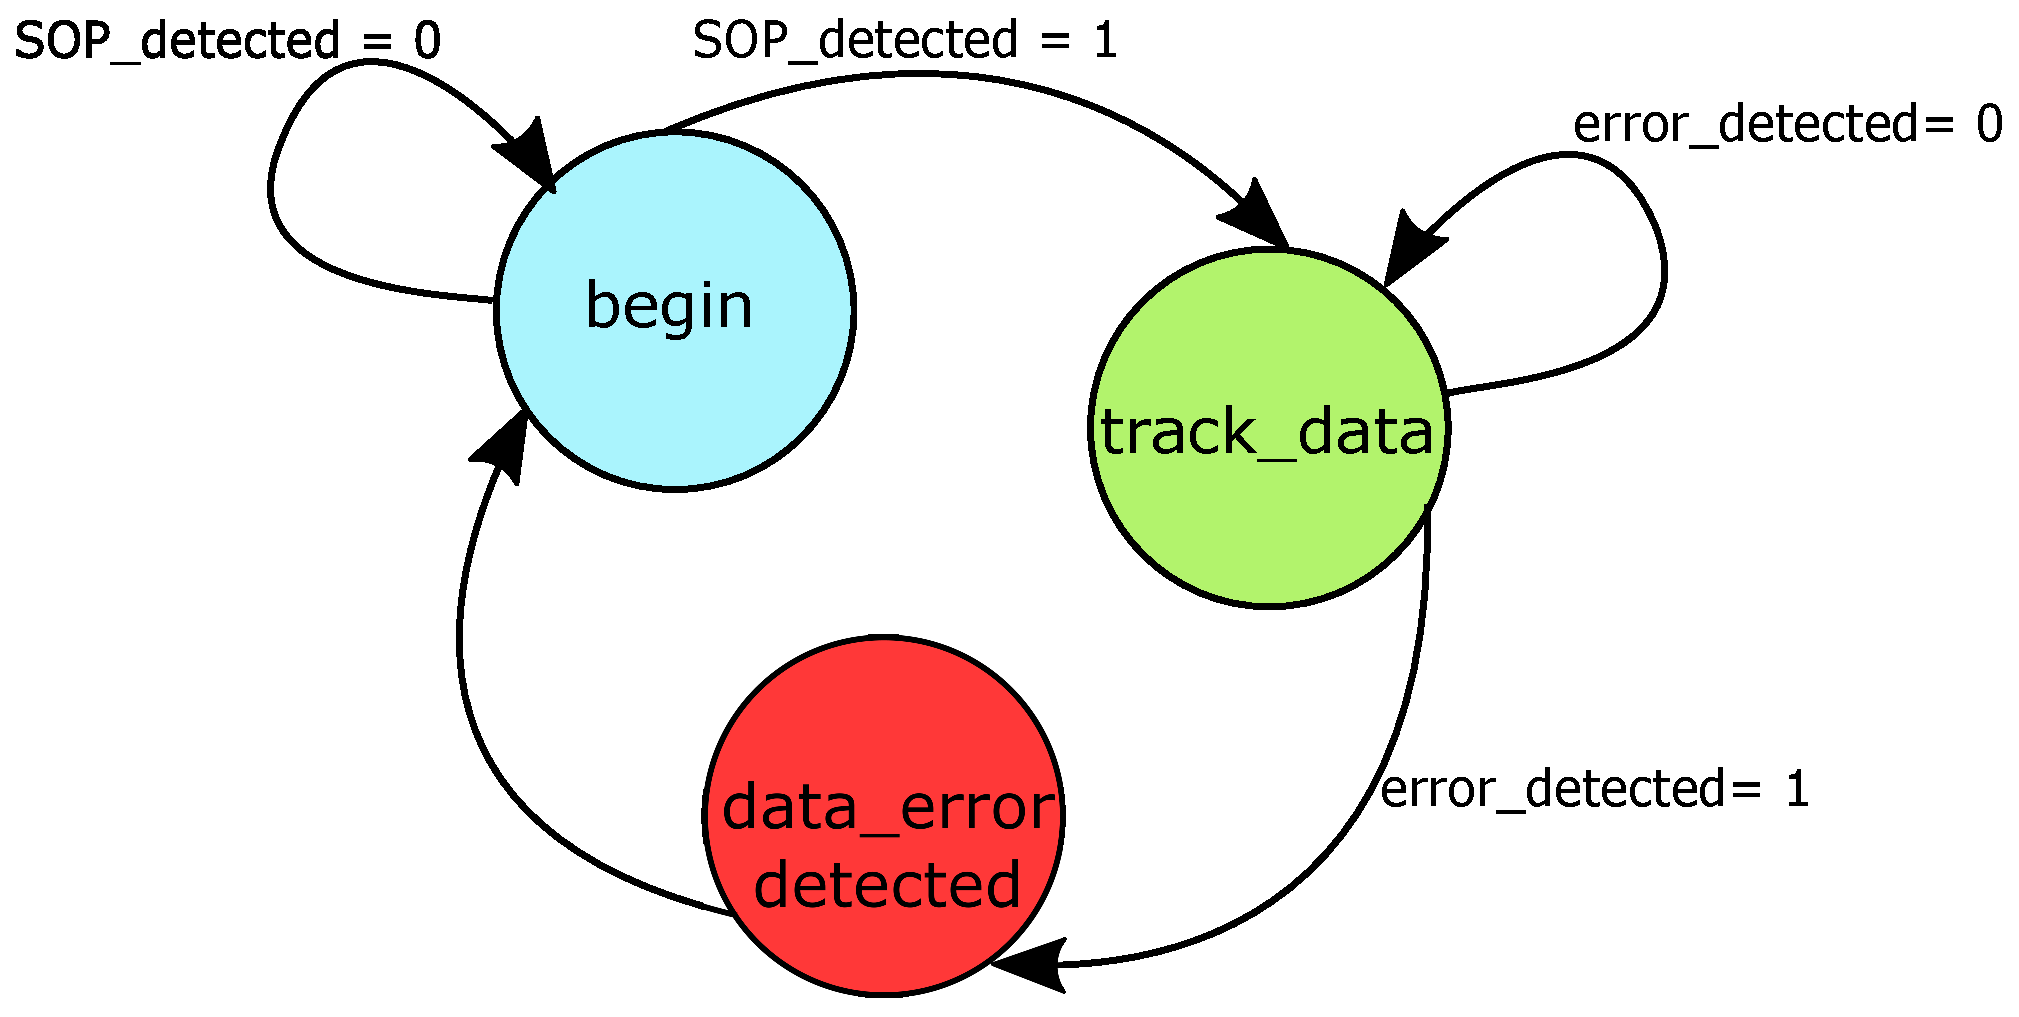
\includegraphics[width=0.8\textwidth]{fsm1}
			\captionsetup{width=1.0\linewidth}
			\caption[Máquina de estados de transmissão]{Máquina de estados de transmissão}
			\label{fig:FSM1}
	\end{center}
	\end{figure}
	
	A figura \ref{fig:FSM1} na página \pageref{fig:FSM1} representa a máquina de estados detalhada anteriormente. De notar que na imagem estão representadas algumas \textit{flags} que decisão de transição, mas que não são mais do que já foi explicado. A \textit{flag} "\textit{SOP\_detected}" indica que se a trama de inicio de pacote foi encontrada nos dados recebidos e "\textit{error\_detected}" indica que foi detetado um erro nos dados recebidos. Ambas são definidas por máquinas de estados que serão explicadas de seguida.
	
	
	\item \textbf{Máquina de leitura de dados}
	 
	 Esta máquina de estados é responsável pela constante procura de dados recebidos pelo recetor. Isto é, os dados vão sendo recebidos e guardados em registos que guardam as duas últimas tramas chegadas do recetor. Isto porque na combinação dessas duas tramas pode-se encontrar a indicação que dá início à transmissão: a trama SOP. Essas duas últimas tramas vão sendo constantemente verificadas sendo o seu conteúdo a motivação para a transição de estados. %Os estados desta máquina passam de seguida a ser descritos:
	 
	 A figura \ref{fig:fsm2} da página \pageref{fig:fsm2} ilustra a máquina de estados referida anteriormente. Contudo antes de descrever a máquina de estados, faz-se uma breve descrição das \textit{flags} de transição de estados presentes na figura:
	 

	 	\begin{figure}[h!]
	 		\begin{center}
	 			\leavevmode
	 			\includegraphics[width=0.8\textwidth]{fsm_track_data}
	 			\captionsetup{width=1.0\linewidth}
	 			\caption[Máquina de estados leitura de dados]{Máquina de estados leitura de dados}
	 			\label{fig:fsm2}
	 		\end{center}
		\end{figure}
	 
	\begin{itemize}
		\item \textit{all\_incoming\_data}: Esta \textit{flag} indica se todos os bits presentes nas duas últimas tramas recebidas no recetor são 0 ou não. Se sim, então a \textit{flag} é igual zero, senão é um.
		
		\item \textit{data\_valid\_detected}: Esta \textit{flag} indica se foi encontrado nos dados recebidos (nas duas últimas tramas) a trama SOP em alguma das situações assinaladas a cinza presentes na figura \ref{fig:alinhamento_tramas_gtx} na página \pageref{fig:alinhamento_tramas_gtx}.
		
		\item \textit{reset}: indica se foi ativado o sinal para repôr os dados originais da máquina de estados.
	\end{itemize}	 
	 
	 Estas são as principais flags de transição de estados da máquina, de seguida serão detalhados todos os estados da mesma:
	 
	 	 \begin{itemize}
	 	\item \textbf{\textit{Waiting}:} Este estado indica que o recetor ainda não está a receber dados, isto porque a \textit{flag} \textit{all\_incoming\_data} está inativa. Por defeito quando não há transmissão de dados do lado do transmissor, o recetor recebe apenas dados iguais a zero. Assim que esta \textit{flag} se ativa então procede-se para o estado de procura da trama de início de transmissão.
	 	
	 	\item \textbf{\textit{Searching}:} Neste estado, a máquina procura pela trama que dá inicio à transmissão de dados (SOP). Uma vez que ela pode vir alinhada em diferentes bytes nas tramas do recetor, então a máquina procura por SOP nas quatro situações difererentes apresentadas na figura \ref{fig:alinhamento_tramas_gtx} na página \pageref{fig:alinhamento_tramas_gtx}. Assim que encontra SOP, memoriza os limites das tramas em que foi esta foi encontrada para que possa de seguida retirar todos os outros dados de transmissão e transita de estado.
	 	
	 	\item \textbf{\textit{Data\_valid}:} Este estado serve essencialmente para guardar os dados devidamente alinhados, uma vez que já foi dado o início de transmissão, segundo os limites da trama SOP. Ativa-se a flag \textit{bit\_align} para que o sistema reconheça que os dados se encontram alinhados. Se os dados que estão a ser guardados em \textit{data\_align} corresponderem à trama SOP então transita-se de estado para indicar que esta trama foi detetada. 
	 	
	 	\item \textbf{\textit{SOP\_detected}:} Quando este estado está ativo, então os dados alinhados correspondem à trama SOP, e por isso deve-se ativar a \textit{flag} "\textit{SOP\_detected}". Este estado mantém-se ativo enquanto os dados alinhados corresponderem à trama SOP e transita para o estado "\textit{data\_valid}" assim que tal deixar de ser verdade. 
	 \end{itemize}
 
 		Sempre que transmissão for interrompida (\textit{all\_incoming\_data} se iguala a zero) ou o sinal de \textit{reset} for ativo (quer por opção do utilizador ou pelo módulo GTX), então a máquina retorna ao estado inicial e repõe os dados originais do sistema. 
	 
	 	Inicialmente o estado ativo é "\textit{waiting}",e todas as \textit{flags} de decisão de mudança de estado (\textit{all\_incoming\_data} e \textit{data\_valid\_detected}) estão igualadas a zero.
	 
	 
	 \item \textbf{Máquina de estados de verificação do alinhamento dos dados}
	
	Tal como já foi mencionado várias vezes ao longo do documento, para taxas de transmissão superiores a 5 Gb/s , o transcetor pode alinhar falsamente os dados. Por esse motivo, as tramas recebidas podem não vir dentro dos limites apresentados na figura \ref{fig:alinhamento_tramas_gtx} na página \pageref{fig:alinhamento_tramas_gtx}, o que leva ao uso de uma máquina de estados que verifique tal.
	
	A máquina de estados apresentada na figura \ref{fig:fsm3} na página \pageref{fig:fsm3} é responsável pela detecção do devido alinhamento das tramas recebidas de acordo com a figura \ref{fig:alinhamento_tramas_gtx} na página \pageref{fig:alinhamento_tramas_gtx}. Caso tal não se verifique, então é também responsável pelo alinhamento manual das tramas.
	
		\begin{figure}[h!]
			\begin{center}
				\leavevmode
				\includegraphics[width=0.9\textwidth]{fsm_bit_align}
				\captionsetup{width=1.0\linewidth}
				\caption[Máquina de estados de verificação do alinhamento dos dados]{Máquina de estados de verificação do alinhamento dos dados}
				\label{fig:fsm3}
		\end{center}
	\end{figure}
	
	%Descrição das flags
	Antes de se passar à descrição de cada estado, é de notar que existem algumas \textit{flags} de decisão de transição de estados:
	\begin{itemize}
		\item \textit{bit\_align}: Esta \textit{flag} indica se a palavra de se encontra devidamente alinhada, tal como ilustrada na figura \ref{fig:alinhamento_tramas_gtx} na página \pageref{fig:alinhamento_tramas_gtx}. 
		
		\item \textit{all\_incoming\_data}: Esta \textit{flag} já foi mencionada e detalhada na máquina de estado que faz a leitura de dados.
		
		\item \textit{count\_slip\_complete}: Esta é uma flag que fica ativa quando um contador termina (será explicado mais à frente).
		
		\item \textit{reset}: Indica a reposição dos dados originais da máquina de estados quando ativa.
	\end{itemize}
	
	%Descrição dos estados
	
	Esta máquina funciona apenas com a utilização de três estados:
	\begin{itemize}
		\item \textbf{\textit{Idle\_slip}:} Este estado é essencialmente uma espera pela chegada de dados e também pela detecção do desalinhamento da palavra. Há transição de estado quando se verifica que as tramas que chegam ao recetor não estão alinhadas de acordo com os limites que deveriam estar.
		
		\item \textbf{\textit{Slip\_assert}:} Este estado está ativo quando há deteção de falso alinhamento de palavras, e por isso ativa-se a saída que liga ao GTX: RXSLIDE. A ativação deste sinal vai permitir que as tramas sejam deslocadas em 1 bit,. Este estado transita imediatamente para o estado de \textit{Wait\_state}.
		
		\item \textbf{\textit{Wait\_state}:} Neste estado o sinal de saída RXSLIDE volta a estar inativo e aguarda-se que a operação de deslocamento de 1 bit se verifique. Como estamos perante um \textit{datapath} de 40 bits, aguarda-se 64 ciclos de relógio. Após esta espera, a flag \textit{count\_slip\_complete} fica ativa e há transição de estado.
	\end{itemize}
	
	De notar que sempre que houver falha de transmissão ou o sinal de \textit{reset} for ativo, então os sinais são repostos para os originais e volta-se ao estado \textit{Idle\_slip}.
	
	%Descrição dos dados originais da maquina
	
	Inicialmente o estado ativo é o {\textit{Idle\_slip} }e as \textit{flags} de sinalização de transição de estado são igualadas a 0.
	
%	\item \textbf{Máquina que deteta os erros }
%	\item \textbf{Máquina que deteta o estado da ligação}
\end{enumerate}

Para além destas máquinas de estados apresentadas, existe a possibilidade de implementação de uma outra que verifique os erros das tramas chegadas. Esta máquina torna-se útil quando há a implementação de códigos detetores de erros nas tramas, ativando a \textit{flag}  "\textit{error\_detected}" sempre que o \textit{checksum} recebido na trama não corresponde à mensagem. Contudo, nesta abordagem inicial tal não é realizado e por isso essa \textit{flag} é globalmente igualada a zero.

Quando os dados estão alinhados, são ainda extraídos da trama recebida os valores de cada sinal a transmitir para a placa HDMI. Quando se recebe uma trama que é igual a SOF iguala-se todos os sinais a zero, no entanto quando a ligação está a procura de dados (o estado \textit{track\_data} está ativo) os dados são extraídos segundo o formato da trama enviada , representada na imagem \ref{fig:trama_abordagem_inicial} na página \pageref{fig:trama_abordagem_inicial}.

\subsubsection*{Bloco de envio de dados para a placa HDMI} \label{subsub:serial_send signals to HDMI}

Este bloco é responsável pela recepção dos dados alinhados provenientes do bloco verificador de tramas e o seu posterior envio para a placa HDMI transmissora. A imagem \ref{fig:sync_block_to_HDMI} na página \pageref{fig:sync_block_to_HDMI} o diagrama de blocos deste módulo.

\begin{figure}[h!]
	\begin{center}
		\leavevmode
		\includegraphics[width=0.5\textwidth]{sync_block_to_HDMI}
		\captionsetup{width=1.0\linewidth}
		\caption[Diagrama de blocos de envio de dados para a placa HDMI transmissora]{Diagrama de blocos de envio de dados para a placa HDMI transmissora}
		\label{fig:sync_block_to_HDMI}
	\end{center}
\end{figure}

Os dados provenientes do bloco anterior são lidos para um registo ao flanco positivo do sinal de relógio que alimenta este módulo (RXUSRCLK2). De seguida, todos os dados presentes nos registos são enviados para a placa HDMI transmissora, incluindo o sinal de relógio RXUSRCLK2

\subsubsection*{Localizações das portas de saída do módulo de topo} \label{subsub:serial_locs_planD}

Na imagem \ref{fig:planD} visualiza-se o diagrama de blocos desenvolvido para esta arquitetura com os seus diversos sub-módulos. 
\begin{figure}[h!]
	\begin{center}
		\leavevmode
		\includegraphics[width=1.0\textwidth]{planod}
		\captionsetup{width=1.0\linewidth}
		\caption[Diagrama de blocos da arquitetura de transmissão em série de uma barra de cores gerada na FPGA]{Diagrama de blocos da arquitetura de transmissão em série de uma barra de cores gerada na FPGA}
		\label{fig:planD}
	\end{center}
\end{figure}

É possível visualizar que este bloco tem diversas entradas e saídas, e por isso para além de todo o código desenvolvido em verilog para estes sub-módulo, é necessário definir as localizações físicas da FPGA para cada porta de entrada e saída. A tabela \ref{table:loc_planD_simples} da página \pageref{table:loc_planD_simples} apresenta todas as portas de entrada e saída existentes no módulo. 

%%%falar das portas todas
\begin{table}[h!]
	\centering
	%\resizebox{\textwidth}{!}{%
		\begin{tabular}{rlll}
			\hline
			\multicolumn{1}{l}{}                  & \multicolumn{1}{c}{\textbf{Sinal}} & \multicolumn{1}{c}{\textbf{LOC na FPGA}} & \multicolumn{1}{c}{\textbf{Banco na FPGA}} \\ \hline
			\multicolumn{1}{r|}{\textbf{Entrada}} & clk\_p                             & E19                                      & 38                                         \\
			\multicolumn{1}{r|}{\textbf{Entrada}} & clk\_n                             & E18                                      & 38                                         \\
			\multicolumn{1}{r|}{\textbf{Entrada}} & reset                              & N41                                      & 19                                         \\
			\multicolumn{1}{r|}{\textbf{Entrada}} & start                              & E42                                      & 19                                         \\
			\multicolumn{1}{r|}{\textbf{Entrada}} & REF\_CLK\_P                        & AF8                                      & 114                                        \\
			\multicolumn{1}{r|}{\textbf{Entrada}} & REF\_CLK\_N                        & AF7                                      & 114                                        \\
			\multicolumn{1}{r|}{\textbf{Entrada}} & RXP\_IN                            & AG6                                      & 114                                        \\
			\multicolumn{1}{r|}{\textbf{Entrada}} & RXN\_IN                            & AG5                                      & 114                                        \\
			\multicolumn{1}{r|}{\textbf{Saída}}   & TXN\_OUT                           & AK3                                      & 114                                        \\
			\multicolumn{1}{r|}{\textbf{Saída}}   & TXP\_OUT                           & AK4                                      & 114                                        \\
			\multicolumn{1}{r|}{\textbf{Saída}}   & begin\_state                       & M38                                      & 19                                         \\
			\multicolumn{1}{r|}{\textbf{Saída}}   & SOF\_detected                      & R42                                      & 19                                         \\
			\multicolumn{1}{r|}{\textbf{Saída}}   & track\_data                        & P42                                      & 19                                         \\
			\multicolumn{1}{r|}{\textbf{Saída}}   & data\_error\_detected              & N38                                      & 19                                         \\
			\multicolumn{1}{r|}{\textbf{Saída}}   & idle\_slip                         & M39                                      & 19                                         \\
			\multicolumn{1}{r|}{\textbf{Saída}}   & wait\_state                        & R40                                      & 19                                         \\
			\multicolumn{1}{r|}{\textbf{Saída}}   & align                              & P40                                      & 19                                         \\
			\multicolumn{1}{r|}{\textbf{Saída}}   & clk\_px                            & E34                                      & 35                                         \\
			\multicolumn{1}{r|}{\textbf{Saída}}   & enable                             & K35                                      & 34                                         \\
			\multicolumn{1}{r|}{\textbf{Saída}}   & hsync                              & M32                                      & 34                                         \\
			\multicolumn{1}{r|}{\textbf{Saída}}   & vsync                              & L31                                      & 34                                         \\
			\multicolumn{1}{r|}{\textbf{Saída}}   & pixel{[}0{]} a pixel {[}29{]}      & Ver Anexo                                & 34 e 35                                    \\ \hline
		\end{tabular}%
%	}
	\caption[Localizações físicas das portas de entrada e saída da arquitetura desenvolvida]{Localizações físicas das portas de entrada e saída da arquitetura desenvolvida}
	\label{table:loc_planD_simples}
\end{table}

As portas de saída que se conectam à placa HDMI transmissora não são descritas com muito detalhe nesta tabela, contudo essa informação encontra-se detalhada na secção \ref{ap3:imagemFPGA_TX} do anexo \ref{ap3:LOCs}.

Existem também umas portas de saída do módulo que estão contempladas na tabela, mas que não estão incluídas na imagem \ref{fig:planD} da página \pageref{fig:planD}. Essas portas têm os nomes de "\textit{begin\_state}", "\textit{SOF\_detected}", "\textit{track\_data}", "\textit{data\_error\_detected }", "\textit{idle\_slip }", "\textit{wait\_state}" e "\textit{align}". São portas provenientes do módulo verificador de tramas e estão conectadas a LED's para ajudar o utilizador a perceber o estado da ligação, pois correspondem aos diferentes estados explicados em \ref{subsub:serial_frameChecker} na página \pageref{subsub:serial_frameChecker}.

%%%falar das constraints físicas

O conteúdo do ficheiro de restrições físicas pode ser encontrado nas secções \ref{ap:fisicas_paraHDMI} e \ref{ap:fisicas_planD} do anexo \ref{ap2:codigo}. Na secção \ref{ap:fisicas_paraHDMI}  encontram-se as retrições relativas ás portas de saída que se conectam à placa HDMI transmissora e a secção \ref{ap:fisicas_planD} corresponde ás restrições físicas das restantes portas desta arquitetura. O conteúdo das restrições temporais desta mesma arquitetura encontra-se na secção \ref{ap:temporais_planD} do anexo \ref{ap2:codigo}.
%
%%%falar das constrainsts temporais
%
\subsubsection{Resultados} \label{subsub:serial_planDresults}

Após síntese e  implementação da arquitetura desenvolvida a FPGA foi devidamente programada com o \textit{bitstream} gerado. Contudo, nesta arquitetura é necessário ter em consideração que o sinal de relógio de referência que se conecta ao GTX é proveniente de um módulo disponível nesta FPGA Virtex-7 com o nome de "\textit{SuperClock2-Module}", e como tal, antes de programar a FPGA com a arquitetura desenvolvida, deve ser programado este módulo para a frequência desejada (148,5 MHz). \textbf{COMO INCLUO ISTO ??????}

Para testar a arquitetura utilizou-se o \textit{setup} que se pode visualizar na figura \ref{fig:planD_setup} da página \pageref{fig:planD_setup}.
\begin{figure}[h!]
	\begin{center}
		\leavevmode
		\includegraphics[width=0.8\textwidth]{planDsch}
		\captionsetup{width=1.0\linewidth}
		\caption[\textit{Setup} de teste da arquitetura]{\textit{Setup} de teste da arquitetura de transmissão de dados em série da barra de cores gerada na FPGA}
		\label{fig:planD_setup}
	\end{center}
\end{figure}

Os resultados obtidos foram os esperados: a transmissão em série foi obtida e visualizou-se uma barra de cores no monitor. Para além disto, quando se desconectam os cabos SMA, a ligação perde-se. Quando se voltam a conectar, a ligação é recuperada.





\subsection{Transmissão de imagem em série entre dispositivos HDMI} \label{sub:planE}

Nesta subsecção é apresentada uma arquitetura de transmissão de imagem em série entre dispositivos HDMI. Serão detalhados todos as fases do desenvolvimento da arquitetura e todas as decisões tomadas e ainda os resultados obtidos relativamente. Esta arquitetura é semelhante à apresentada na subsecção \ref{sub:planD} na página \pageref{sub:planD} e por isso muitos dos blocos usados nesta são idênticos aos anteriormente apresentados.

\subsubsection{Considerações sobre a arquitetura} \label{subsub:planE_considerações}

A arquitetura desenvolvida gera uma barra de cores em \textit{FULL HD} na FPGA, tal como anteriormente, e ao mesmo tempo recebe os dados provenientes da placa HDMI recetora. Tal como se visualiza na figura \ref{fig:planE_simples} na página \pageref{fig:planE_simples}, os dados a ser transmitidos vão depender do valor de "\textit{start}". Este sinal define a seleção do multiplexador que se visualiza na imagem: se estiver ativo selecciona os dados provenientes do módulo gerador da barra de cores, se estiver inativo os dados seleccionados pelo multiplexador são os dados provenientes da placa HDMI recetora.

\begin{figure}[h!]
	\begin{center}
		\leavevmode
		\includegraphics[width=1.0\textwidth]{planoE_simples_pt}
		\captionsetup{width=1.0\linewidth}
		\caption[Diagrama geral da arquitetura de transmissão em série de imagem entre dispositivos HDMI]{Diagrama geral da arquitetura de transmissão em série de imagem entre dispositivos HDMI}
		\label{fig:planE_simples}
	\end{center}
\end{figure}


\subsubsection{Concepção e Desenvolvimento}

Através da visualização do diagrama blocos simplificado apresentado na imagem \ref{fig:planE_simples} é possivel concluir que o único sub-módulo adicionado é o bloco recetor de dados HDMI. Todos os outros sub-módulos são exatamente iguais ao da arquitetura anterior. Estes sub-módulos estão todos detalhados na subsecção \ref{sub:planD} na página \pageref{sub:planD}. Assim sendo, apenas será detalhado nesta subsecção esse mesmo bloco.

\subsubsection*{Bloco Recetor de dados HDMI}
%explicar o que faz
O bloco recetor de dados HDMI apenas recebe os dados provenientes da placa HDMI recetora e guarda-os em registos síncronos com o flanco positivo do sinal de relógio proveniente do HDMI. O diagrama de blocos deste módulo visualiza-se na imagem \ref{fig:recetorHDMI} da página \pageref{fig:recetorHDMI}.
%explicar o porque de ser necessário
\begin{figure}[h!]
	\begin{center}
		\leavevmode
		\includegraphics[width=0.5\textwidth]{recetorHDMI}
		\captionsetup{width=1.0\linewidth}
		\caption[Bloco recetor de dados HDMI]{Bloco Recetor de dados HDMI}
		\label{fig:recetorHDMI}
	\end{center}
\end{figure}

É de relembrar que existem dois domínios de relógio principais quando se faz a transmissão de dados entre a placa HDMI recetora para o transcetor GTX: o sinal de relógio proveniente da placa HDMI e o sinal de relógio proveniente do transcetor. Apesar de já existir um bloco responsável pela sincronização de dados do domínio do sinal de relógio TXUSRCLK2, o autor de \cite{R024} recomenda que também haja sincronização do lado do domínio que envia os dados. Apesar de as saídas da placa HDMI serem amostradas a uma determinada cadência, segundo os manuais das mesmas (\cite{R009}, \cite{R014} e \cite{R013}), pode existir algum desfasamento de dados que possa vir a provocar meta-estabilidade. Assim sendo, optou-se por criar este bloco.

\subsubsection*{Localizações das portas de saída do módulo de topo} \label{subsub:serial_locs_planE}


\begin{table}[h!]
	\centering
	\begin{tabular}{rlll}
		\hline
		\multicolumn{1}{l}{}                  & \multicolumn{1}{c}{\textbf{Sinal}}     & \multicolumn{1}{c}{\textbf{LOC na FPGA}} & \multicolumn{1}{c}{\textbf{Banco na FPGA}} \\ \hline
		\multicolumn{1}{r|}{\textbf{Entrada}} & clk\_p                                 & E19                                      & 38                                         \\
		\multicolumn{1}{r|}{\textbf{Entrada}} & clk\_n                                 & E18                                      & 38                                         \\
		\multicolumn{1}{r|}{\textbf{Entrada}} & reset                                  & N41                                      & 19                                         \\
		\multicolumn{1}{r|}{\textbf{Entrada}} & start                                  & E42                                      & 19                                         \\
		\multicolumn{1}{r|}{\textbf{Entrada}} & REF\_CLK\_P                            & AF8                                      & 114                                        \\
		\multicolumn{1}{r|}{\textbf{Entrada}} & REF\_CLK\_N                            & AF7                                      & 114                                        \\
		\multicolumn{1}{r|}{\textbf{Entrada}} & RXP\_IN                                & AG6                                      & 114                                        \\
		\multicolumn{1}{r|}{\textbf{Entrada}} & RXN\_IN                                & AG5                                      & 114                                        \\
		\multicolumn{1}{r|}{\textbf{Entrada}} & clk\_px\_in                            & AJ32                                     & 14                                         \\
		\multicolumn{1}{r|}{\textbf{Entrada}} & enable\_in                             & AN38                                     & 15                                         \\
		\multicolumn{1}{r|}{\textbf{Entrada}} & hsync\_in                              & AU39                                     & 15                                         \\
		\multicolumn{1}{r|}{\textbf{Entrada}} & vsync\_in                              & AU38                                     & 15                                         \\
		\multicolumn{1}{r|}{\textbf{Entrada}} & pixel\_in {[}0{]} a pixel\_in {[}29{]} & Ver Anexo                                & 14 e 15                                    \\
		\multicolumn{1}{r|}{\textbf{Saída}}   & TXN\_OUT                               & AK3                                      & 114                                        \\
		\multicolumn{1}{r|}{\textbf{Saída}}   & TXP\_OUT                               & AK4                                      & 114                                        \\
		\multicolumn{1}{r|}{\textbf{Saída}}   & begin\_state                           & M38                                      & 19                                         \\
		\multicolumn{1}{r|}{\textbf{Saída}}   & SOF\_detected                          & R42                                      & 19                                         \\
		\multicolumn{1}{r|}{\textbf{Saída}}   & track\_data                            & P42                                      & 19                                         \\
		\multicolumn{1}{r|}{\textbf{Saída}}   & data\_error\_detected                  & N38                                      & 19                                         \\
		\multicolumn{1}{r|}{\textbf{Saída}}   & idle\_slip                             & M39                                      & 19                                         \\
		\multicolumn{1}{r|}{\textbf{Saída}}   & wait\_state                            & R40                                      & 19                                         \\
		\multicolumn{1}{r|}{\textbf{Saída}}   & align                                  & P40                                      & 19                                         \\
		\multicolumn{1}{r|}{\textbf{Saída}}   & clk\_px                                & E34                                      & 35                                         \\
		\multicolumn{1}{r|}{\textbf{Saída}}   & enable                                 & K35                                      & 34                                         \\
		\multicolumn{1}{r|}{\textbf{Saída}}   & hsync                                  & M32                                      & 34                                         \\
		\multicolumn{1}{r|}{\textbf{Saída}}   & vsync                                  & L31                                      & 34                                         \\
		\multicolumn{1}{r|}{\textbf{Saída}}   & pixel{[}0{]} a pixel {[}29{]}          & Ver Anexo                                & 34 e 35                                    \\ \hline
	\end{tabular}
	\caption{Localizações físicas das portas de entrada e saída da arquitetura}
	\label{table:LOC_simples_planE}
\end{table}



\begin{figure}[h!]
	\begin{center}
		\leavevmode
		\includegraphics[width=1.0\textwidth]{planoE}
		\captionsetup{width=1.0\linewidth}
		\caption[Diagrama de blocos da arquitetura de transmissão de imagem em série]{Diagrama de blocos da arquitetura de transmissão de imagem em série}
		\label{fig:recetorHDMI}
	\end{center}
\end{figure}

\subsubsection{Resultados} \label{subsub:serial_planEresults}